\documentclass[parskip=full]{scrartcl}
\usepackage[T1]{fontenc}    % avoid garbled Unicode text in pdf
\usepackage[utf8]{inputenc} % use utf8 file encoding for TeX sources
\usepackage[german]{babel}  % german hyphenation, quotes, etc
\usepackage{hyperref}       % detailed hyperlink/pdf configuration
\hypersetup{                % ‘texdoc hyperref‘ for options
pdftitle={PSE: Entwicklung eines relationalen Debuggers - Pflichtenheft},%
,%
}
\usepackage{graphicx}       % provides commands for including figures
\usepackage{csquotes}       % provides \enquote{} macro for "quotes"
\usepackage[nonumberlist]{glossaries}     % provides glossary commands
\usepackage{enumitem}

\makenoidxglossaries


\title{PSE:\\ Entwicklung eines relationalen Debuggers\\ Pflichtenheft}
\author{
	Benedikt Wagner\\
	\texttt{udpto@student.kit.edu}
	\and Chiara Staudenmaier\\
	\texttt{uzhtd@student.kit.edu}
	\and Etienne Brunner\\
	\texttt{urmlp@student.kit.edu}
	\and Joana Plewnia\\
	\texttt{uhfpm@student.kit.edu} 
	\and Pascal Zwick\\
	\texttt{uyqpk@student.kit.edu}
	\and Ulla Scheler\\
	\texttt{ujuhe@student.kit.edu}
}

\begin{document}

\maketitle
\newpage

\tableofcontents
\newpage

\section{Produktübersicht}
%kurze Übersicht über das Produkt
Das Produkt soll dem Nutzer die Möglichkeit bieten, mehr als ein Programm gleichzeitig zu debuggen und interaktiv zu analysieren. Dabei sollen die Konzepte eines herkömmlichen Debuggers, namentlich Einzelschritte, Breakpoints und Variableninspektion, erhalten bleiben und um zusätzliche Konzepte, die den Umgang mit zwei Programmläufen erleichtern, erweitert werden. Der Fokus liegt hierbei auf der Unterstützung des Findens von relationalen Zusammenhängen in den vom Nutzer in einer WHILE-Sprache verfassten Programmen.


\section{Produkteinsatz}
Das Produkt unterstützt das Institut für theoretische Informatik am Karlsruher Institut für Technologie beim Führen von Beweisen zu relationalen Eigenschaften von Programmen. Hierbei soll die Möglichkeit des gleichzeitigen Debuggens der Programme dem Nutzer bei der Beweisführung helfen. \\
Verwendet wird das Produkt hierbei von wissenschaftlichen Mitarbeitern am Lehrstuhl "Anwendungsorientierte formale Verifikation - Prof. Dr. Beckert" des Instituts für theoretische Informatik am Karlsruher Institut für Technologie und soll in deren Büroumgebung zum Einsatz kommen.
%Betriebsbedingungen? Einsatz wo? (Büroumgebung?)

%Anwendungsbereiche, Zielgruppen, Betriebsbedingungen
 

\section{Produktumgebung}
%Software, Hardware, Orgware, Schnittstellen
Das Produkt läuft auf dem Rechner des Nutzers und benötigt keine Kommunikation mit außerhalb. Hierbei läuft das Produkt eventuell neben anderen Applikationen, kommuniziert jedoch nicht mit diesen.

\subsection{Software}
Da es sich bei dem Produkt um ein Java-Programm handelt, muss ein JRE (Java Runtime Environment) auf dem Rechner vorhanden sein oder mitinstalliert werden. \\
Das Produkt läuft sowohl auf Windows, als auch auf Mac OS und Linux.

\subsection{Hardware}
An die Hardware des Rechners werden keine speziellen Anforderungen gestellt. Das Produkt läuft auf jedem Standardrechner (ca. 1 GHz und 128 MB RAM).

\subsection{Schnittstellen}
Das Produkt hat (öffentliche?) Schnittstellen zur graphischen Benutzeroberfläche und zum Interpreter, um diese leicht austauschbar zu gestalten.


\section{Produktfuntionen}
	 	\subsection{Funktionale Anforderungen}
 		\subsubsection{Musskriterien}
		\begin{itemize}
		\item[/FA10/] Im Debugmodus kann der Benutzer Schritte durchführen, um das Programm weiter zu debuggen.
		\item[/FA15/] Durch Einzelschritte können einzelne Programme unabhängig weiter debuggt werden.
		\item[/FA20/] Der Benutzer kann Breakpoints an Zeilen im Code setzen.
		\item[/FA30/] --Programmname-- ist ein Debugger für Quellcodes, welche in der im Kapitel Ergänzungen spezifizierten Sprache geschrieben sind.
		\item[/FA40/] Der Benutzer kann die Schrittgröße manuell festlegen.
		\item[/FA50/] Der Benutzer kann relationale Eigenschaften bezüglich Variablen als Watch-Expressions festlegen.
		\item[/FA60/] Der Benutzer kann relationale Eigenschaften bezüglich Variablen als bedingte Breakpoints festlegen.
		\item[/FA70/] Nach jedem Schritt oder Breakpoint werden die aktuellen Variablenbelegungen angezeigt.
		\item[/FA80/] Im Debugmodus kann der Benutzer durch Auswahl der Option Weiter das Programm bis zum nächsten Breakpoint debuggen.
		\item[/FA90/]--Programmname-- bietet die Möglichkeit, eine Konfigurationsdatei für einen Lauf zu speichern. Diese beinhaltet festgelegte Eingabewerte, Breakpoints, Watch-Expressions, Schrittgröße und die zu debuggenden Codes.
		\item[/FA100/] Das zu debuggende Programm kann direkt in die Textbox des Tools kopiert oder geschrieben werden.
		\item[/FA110/] Das zu debuggende Programm kann aus einer Textdatei eingebunden werden.
		\item[/FA120/] Der Debugmodus kann vom Benutzer abgebrochen werden. Dadurch kehrt der Benutzer zum Editiermodus zurück.
		\item[/FA130/] Die Variablenreihenfolge im Variableninspektor ist manuell veränderbar.
		\end{itemize}
		..
 		\subsubsection{Sollkriterien}
		\begin{itemize}
		\item[/FA200/] Watch-Expressions können auch nur in von Benutzer festgeletem Bereich überprüft werden.
		\item[/FA210/] Variablen im Variableninspektor können ausgeblendet werden.
		\item[/FA220/] Zufällige Vorschläge für Eingabewerte über Vorschlag-Button.
		\item[/FA230/] Jeder angenommene Wert von vom Benutzer ausgewählten Variablen kann gespeichert werden.
		\item[/FA240/] Bei Endlosschleifen wird automatisch abgebrochen. Die maximale Anzahl Schleifendurchläufe kann vom Benutzer festgelegt werden (maximal 250).
		\item[/FA250/] Es können mehr als 2 Programme debuggt werden.
		\end{itemize}
		..
 		\subsubsection{Kannkriterien}
 		..
 		\subsubsection{Abgrenzungskriterien}
	\subsection{Nichtfunktionale Anforderungen}
		\subsubsection{Produktdaten}
			\paragraph{/PD10/ Konfigurationsdateien:}
			Diese Dateien speichern eine Konfiguration des Debuggers.
			Zu diesen gehören die Eingabewerte, Schrittgrößen, Variablen Auswahl, 						Quelltext und Position beider Programme, aber nicht die Ausgabewerte, da diese 			vom Programmcode zur Laufzeit generiert werden.
			Weiter müssen alle Breakpoints gespeichert werden. Dazu zählen sowohl gesetzte 			als auch bedingte Breakpoints. Letzteres benötigt keine Speicherung der Zeile, 			sondern eines Bereiches, zweier Variablen der Programmtexte und eines Operators. 				Dies gilt auch für die Watch-Expressions mit Ausnahme eines Bereiches.
			\paragraph{/PD20/ Sprachdateien:}
			Diese Datei speichert die Übersetzung der gesamten Benutzeroberfläche.
			Dazu gehören die Texte auf GUI-Elementen und Tooltips.
			\paragraph{/PD30/ Einstellungsdatei:}
			Diese Datei speichert die zuletzt ausgewählte Sprache und die URL der 						Konfigurationsdatei, welche zur zuletzt verwendeten Konfiguration passt.
		\subsubsection{Produktleistungen}
		..
		\subsubsection{Weitere nichtfunktionale Anforderungen}
		..

\section{Qualitätsanforderungen}
..

\newpage
\section{Anwendungsfälle und Szenarien}
\begin{figure}[h] 
  \centering
     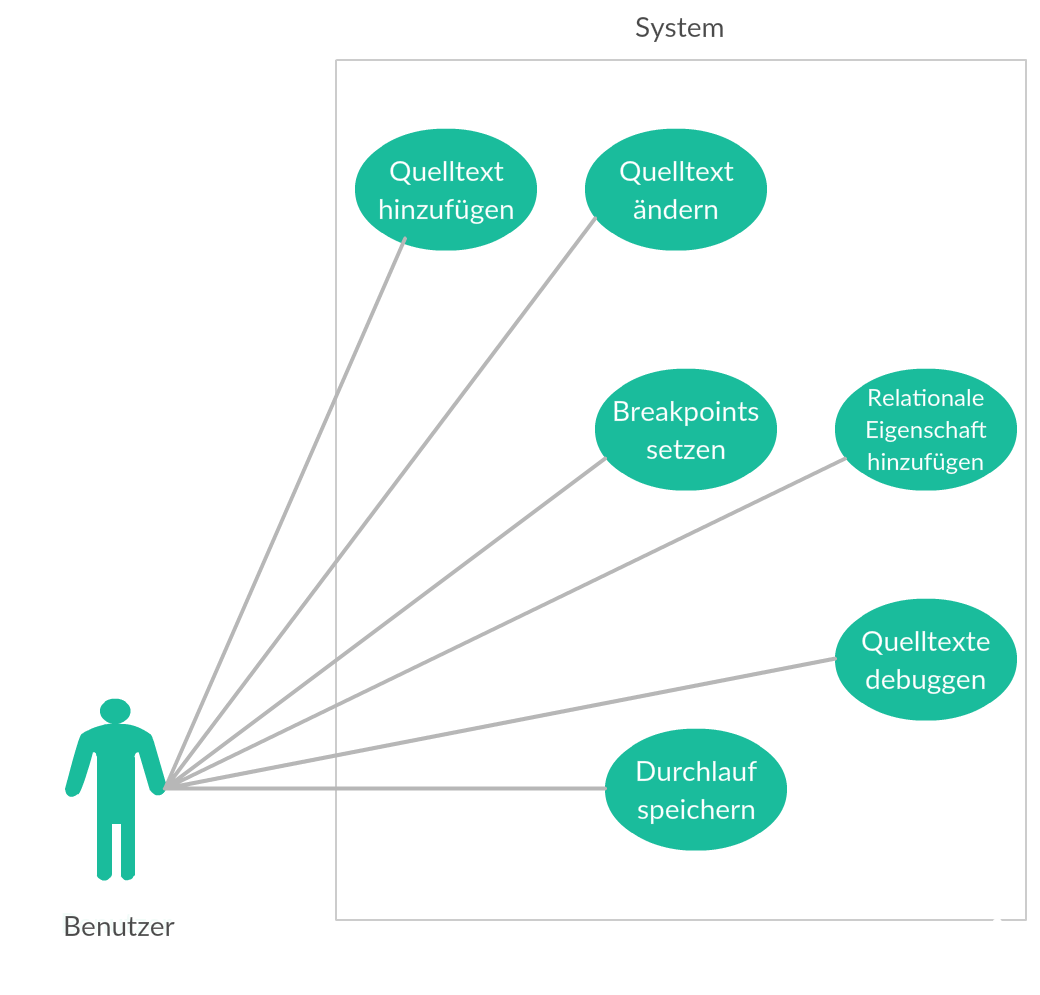
\includegraphics[width=0.7\textwidth]{Anwendungsfalldiagramm}
  \caption{Anwendungsfalldiagramm}
  \label{fig:Bild1}
\end{figure}

\section{Globale Testfälle}
..

\newpage
\section{Systemmodelle}
%Architektur, Verhalten, usw
\begin{figure}[h] 
  \centering
     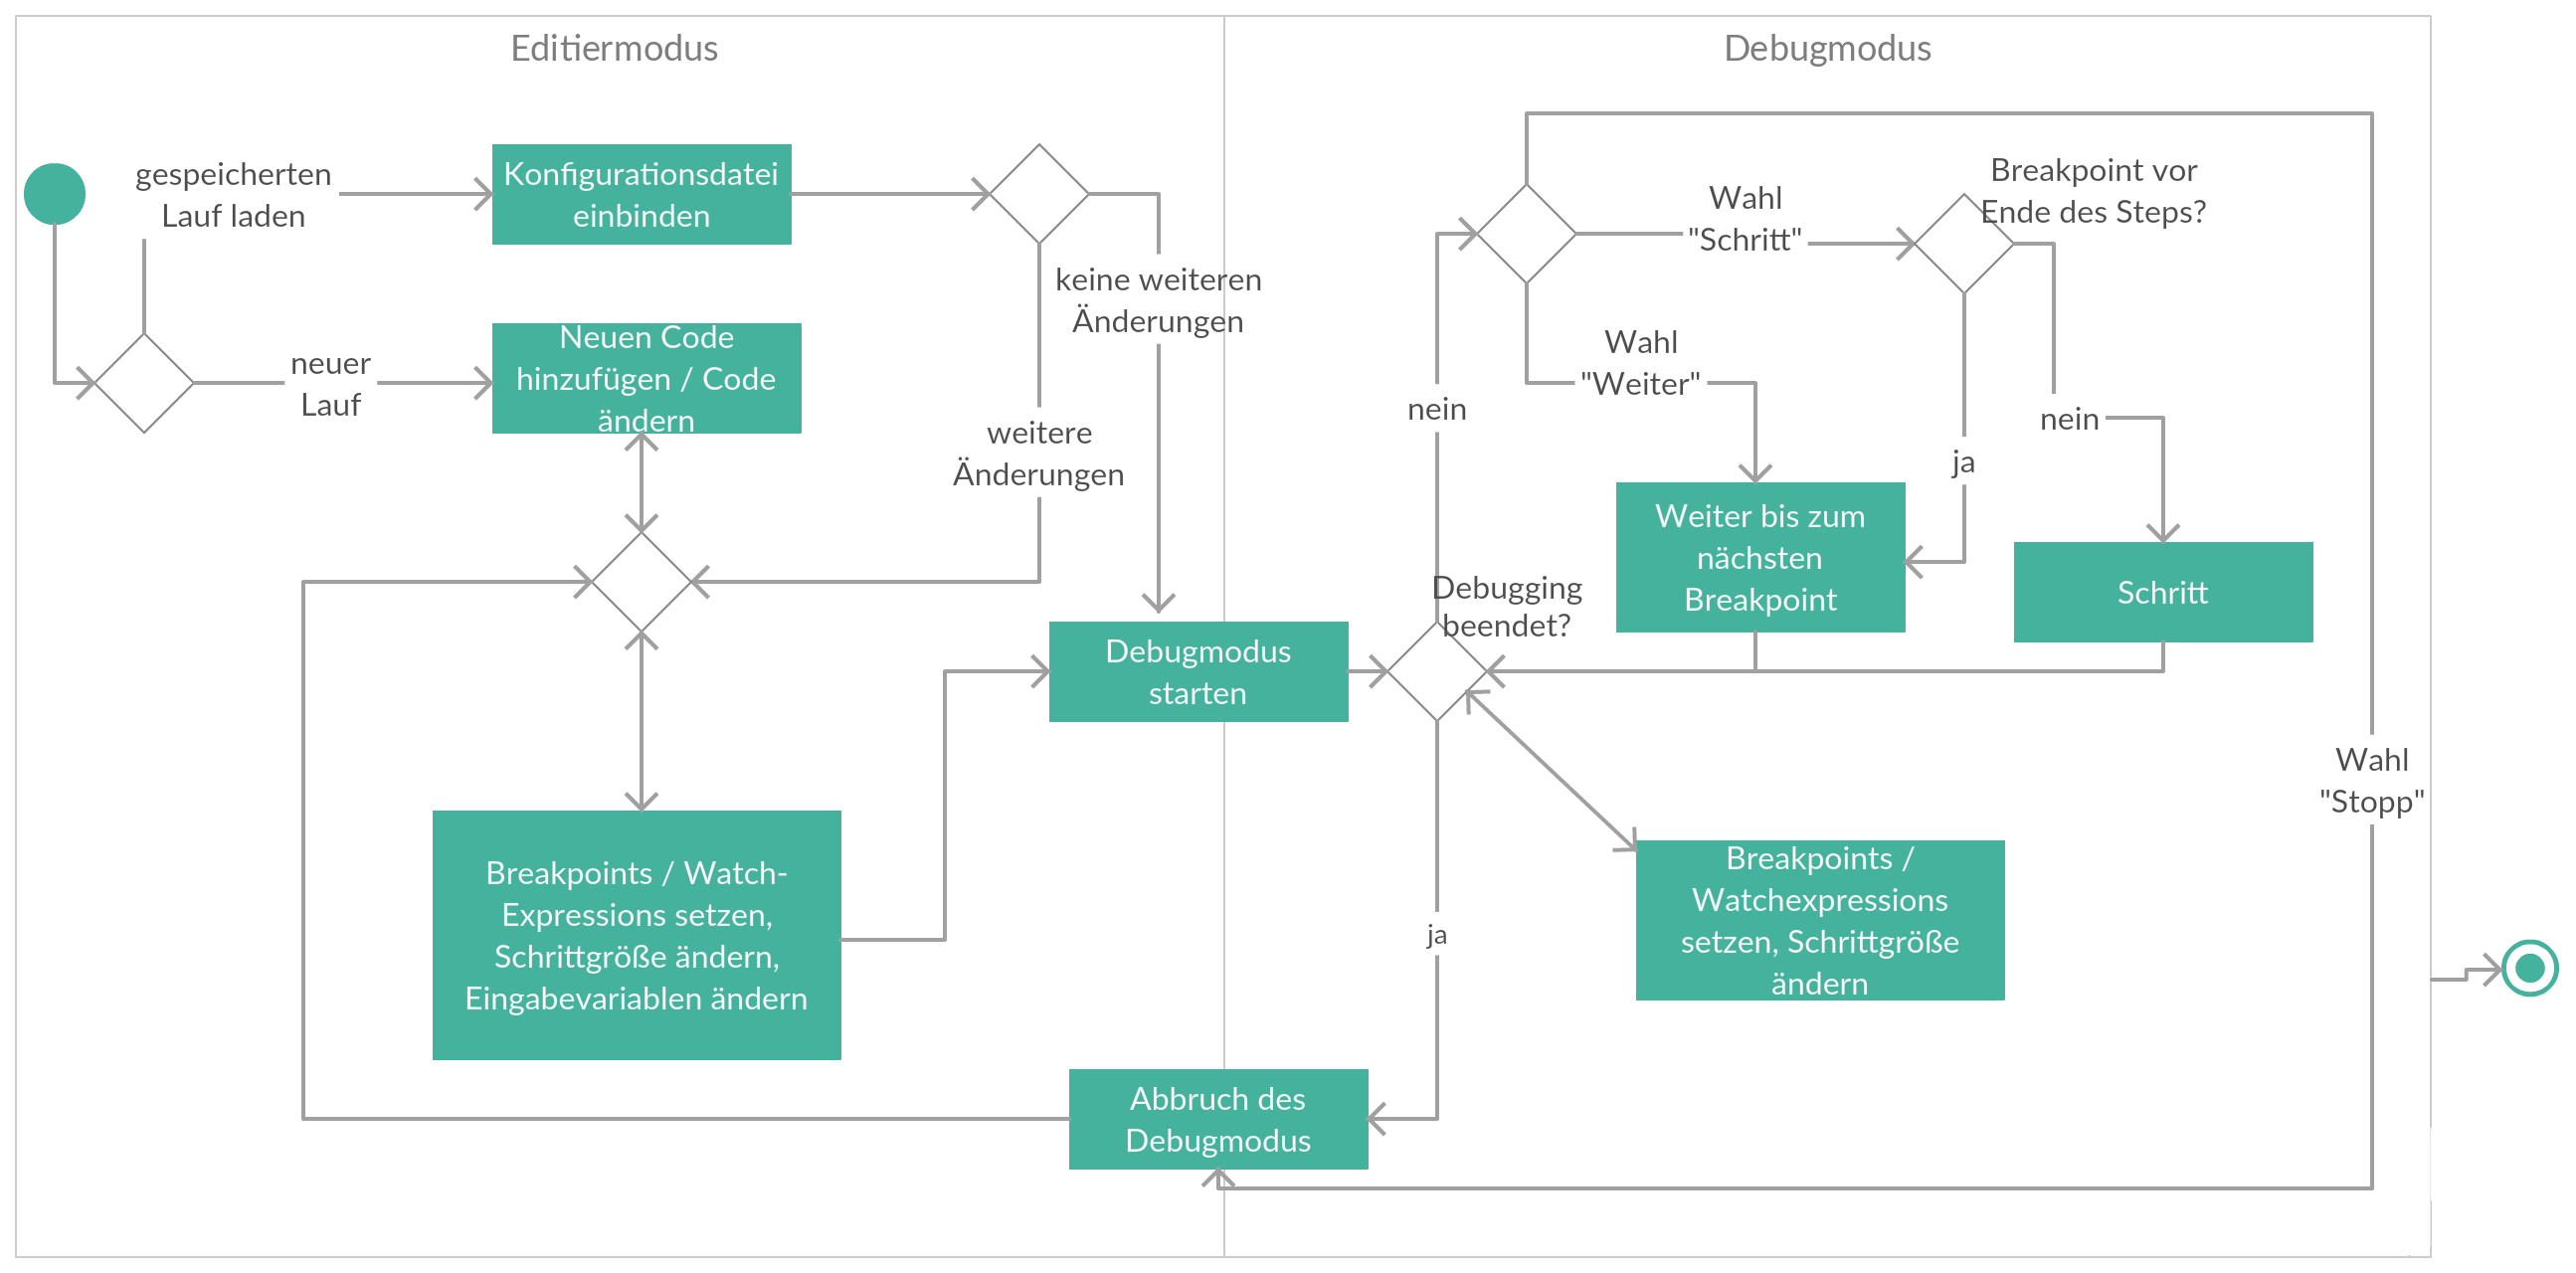
\includegraphics[width=0.9\textwidth]{Aktivitaetsdiagramm}
  \caption{Aktivitätsdiagramm}
  \label{fig:Bild1}
\end{figure}

\newpage
\section{Benutzungsoberfläche}
%Gui-Skizzen, Erklärungen der Menüs, usw
\begin{figure}[!ht] 
    \vspace{-10pt}
    \centering
       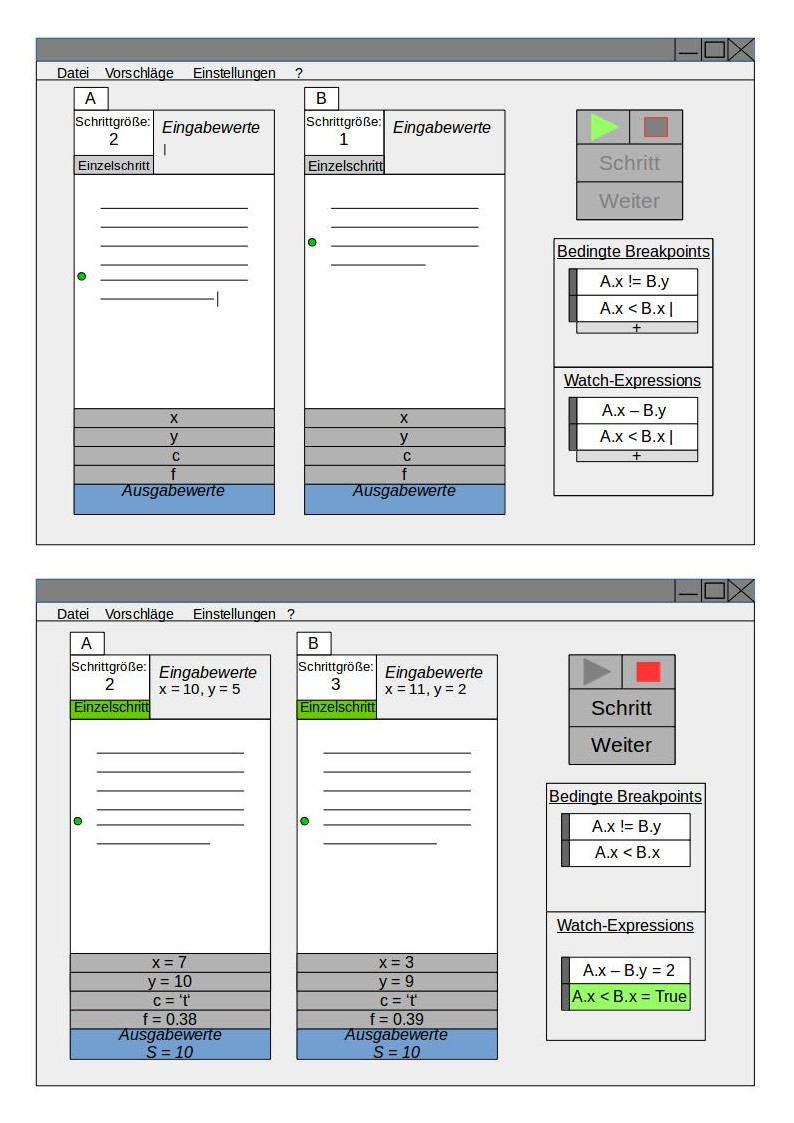
\includegraphics[width=0.7\textwidth]{skizzeFull.jpg}
       \caption{
         Benutzeroberfläche von --Programmname-- im Editiermodus (oben) und im Debugmodus
         (unten)
       }
    \label{fig:Bild1}
\end{figure}

    \subsection{Beschreibung}
        Befindet sich --Programmname-- im Editiermodus, so können die Eingabequelltexte über die 
        Eingabefenster bearbeitet werden.
        Durch Verändern des Textes im Bereich \enquote{Eingabewerte} können Werte der Eingangsvariablen
        spezifiziert, gelöscht und verändert werden. 
        Bedingte Haltepunkte und Watch-Expressions können durch Betätigung der jeweiligen 
        \enquote{+}-Schaltflächen hinzugefügt werden.
        Die Schaltflächen \enquote{Schritt} und \enquote{Weiter}, sowie \enquote{Einzelschritt} können nicht betätigt
        werden. Betätigung der Schaltfläche mit dem grünen Pfeil verursacht den Übergang von
        --Programmname-- in den Debugmodus.
        
        Befindet sich --Programmname-- im Debugmodus, können die Eingabequelltexte nicht
        über die Eingabefenster bearbeitet werden. Die \enquote{+}-Schaltflächen für bedingte Haltepunkte
        und Watch-Expressions können nicht betätigt werden.
        Die Schaltflächen \enquote{Schritt}, \enquote{Weiter} und \enquote{Einzelschritt} können betätigt werden.
        Betätigung der Schaltfläche mit dem roten Viereck verursacht den Übergang von --Programmname-- in den Editiermodus.
        
        
\section{Zeit- und Ressourcenplanung}
..

\section{Ergänzungen}
..

\section{Glossar}




\end{document}
\grid
